%%%%%%%%%%%%%%%%%%%%%%%%%%%%%%%%%%%%%%%%%%%%%%%%%%
\chapter{Introducción}

%%%%%%%%%%%%%%%%%%%%%%%%%%%%%%%%%%%%%%%%%%%%%%%%%%
\section{Lenguajes interpretados o de
  \emph{scripting}\index{scripting}}

Un script o guión es una serie de órdenes que se pasan a un
intérprete\index{intérprete} para que las ejecute. No cumplen la
definición de programa porque no son ejecutables por ellos mismos. Un
programa se comunica directamente con el sistema operativo mientras
que un script lo hace con un intérprete que a su vez envía comandos al
sistema operativo. En este proceso de comunicación \textbf{el programa
no es el script, el archivo de código, sino el intérprete} que lee
línea por línea el código y que no ejecuta la siguiente orden hasta
que no ha terminado con la anterior.

Esta es la diferencia entre los lenguajes basados en código fuente de
los lenguajes de scripting. Los primeros son C, C++, Fortran, Ada,
Cobol, Pascal... El código fuente escrito es transformado por un
compilador\index{compilador} en un archivo ejecutable binario que sólo
es capaz de entender el ordenador.

Los lenguajes de scripting más conocidos son, en el caso de los
lenguajes de uso general, Java, Python y Ruby. La popularidad de Java
se debe a su naturaleza de producto comercial muy sencillo de
administrar mientras que Python y Ruby son Software Libre; de igual o
más calidad pero sin publicidad.  Python es un lenguaje basado en la
consistencia que ofrece una gran productividad y versatilidad.  Ruby
es uno de los lenguajes más recientes, su popularidad está aumentando
gracias a la aplicación Ruby on Rails orientada al desarrollo de
páginas web.

Existe una gran variedad en los lenguajes de scripting orientado a
matemáticas. Matlab, Maple, Mathematica, Scilab, Octave, Euler,
O-Matrix, R o S son lenguajes de scripting.  Los más conocidos son
Matlab, Mathematica y Maple.

No debemos considerar Matlab como únicamente un producto. El scripting
científico es una gran herramienta que hay que dominar
independientemente del programa. Una vez hayamos aprendido a usar
Matlab es posible que se tengamos que aprender a utilizar R, orientado
a análisis de datos, o Scilab si trabajamos en Francia.


\section{Un lenguaje de scripting científico, Matlab\index{Matlab}.}

Un lenguaje interpretado se parece a una herramienta que todos
conocemos perfectamente, una calculadora. Es incomprensible como
alguien se siente completamente cómodo delante de una cajita con una
pantalla y muchas teclas y en cambio le invade el miedo delante de una
consola como la de la figura \ref{cap:Esta-es-una}:

%
\begin{figure}[h]
  \centering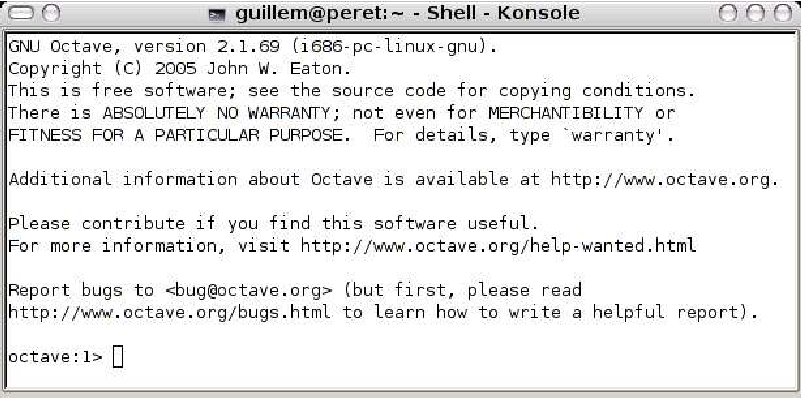
\includegraphics[%
  width=14cm,
  keepaspectratio]{figuras/octave}


  \caption{\label{cap:Esta-es-una}Esta es una consola Linux, mucho más
    útil que el Command Prompt de Windows}
\end{figure}


Si hacemos el esfuerzo de abstracción y simplificamos la ventana
anterior nos queda el símbolo de entrada:

\begin{verbatim}
>>
\end{verbatim}
¿Qué hacemos a parte de quedarnos paralizados? Pues si esto es una
calculadora vamos a usarlo como una calculadora:


\begin{lstlisting}
>> 2+2
ans = 4  
\end{lstlisting}


Este ejemplo no sirve para nada pero resume perfectamente el uso de
Matlab. En el fondo es una calculadora programable con unas
posibilidades casi infinitas. Si a esto se suma un lenguaje intuitivo
y una gran biblioteca de funciones el resultado es una herramienta
verdaderamente útil para ingenieros y científicos.

Esta manera de trabajar no es un invento de Matlab, los lenguajes
interpretados ya existían mucho antes. Lo que sí es novedoso es basar
la arquitectura del lenguaje en conceptos matemáticos; entre ellos uno
muy importante: la función. Mientras los lenguajes clásicos se basan
en subrutinas o objetos Matlab dispone de una biblioteca formada
exclusivamente por funciones. Este diseño tan simple es lo que ha
llevado Matlab a su éxito, es un acercamiento matemático a la
programación orientada a matemáticas. Si queremos calcular el seno de
$\frac{\pi}{2}$ lo que haremos será llamar a la función como se haría
sobre el papel:

\begin{lstlisting}
>> sin(pi/2)
ans = 1
\end{lstlisting}
Entonces nada impide usar el mismo concepto para resolver problemas
mucho más complejos:

\begin{lstlisting}
>> quad(@(x) besselj(2.5,x),0,4.5)
ans = 1.1178
\end{lstlisting}
Acabamos de hacer la siguiente integral de la función real de Bessel
de primera especie:

$$\int_{0}^{4.5}J_{2.5}(x)dx$$

\texttt{quad} y \texttt{besselj} son funciones que se
han compuesto del mismo modo que se compondrían funciones matemáticas.
Esta línea de código puede ser incomprensible pero al final la
entenderemos con todos los detalles.


\section{El entorno de desarrollo Matlab.}

Matlab como programa no se limita a un intérprete en una consola, es
un entorno de desarrollo al completo. Al iniciar Matlab nos aparecerá
la ventana principal con la consola, el navegador de variables y el
historial de comandos (figura \ref{cap:Ventana-principal-Matlab})%
\footnote{En Unix Matlab puede funcionar también desde el intérprete
de comandos mediante la función \texttt{-nojvm}.  Es una opción interesante
cunando no hemos instalado ninguna máquina virtual de Java}. Evidentemente
lo más importante es la consola; todo lo demás, aunque útil, es prescindible.


\begin{figure}[h]
  \centering{}

  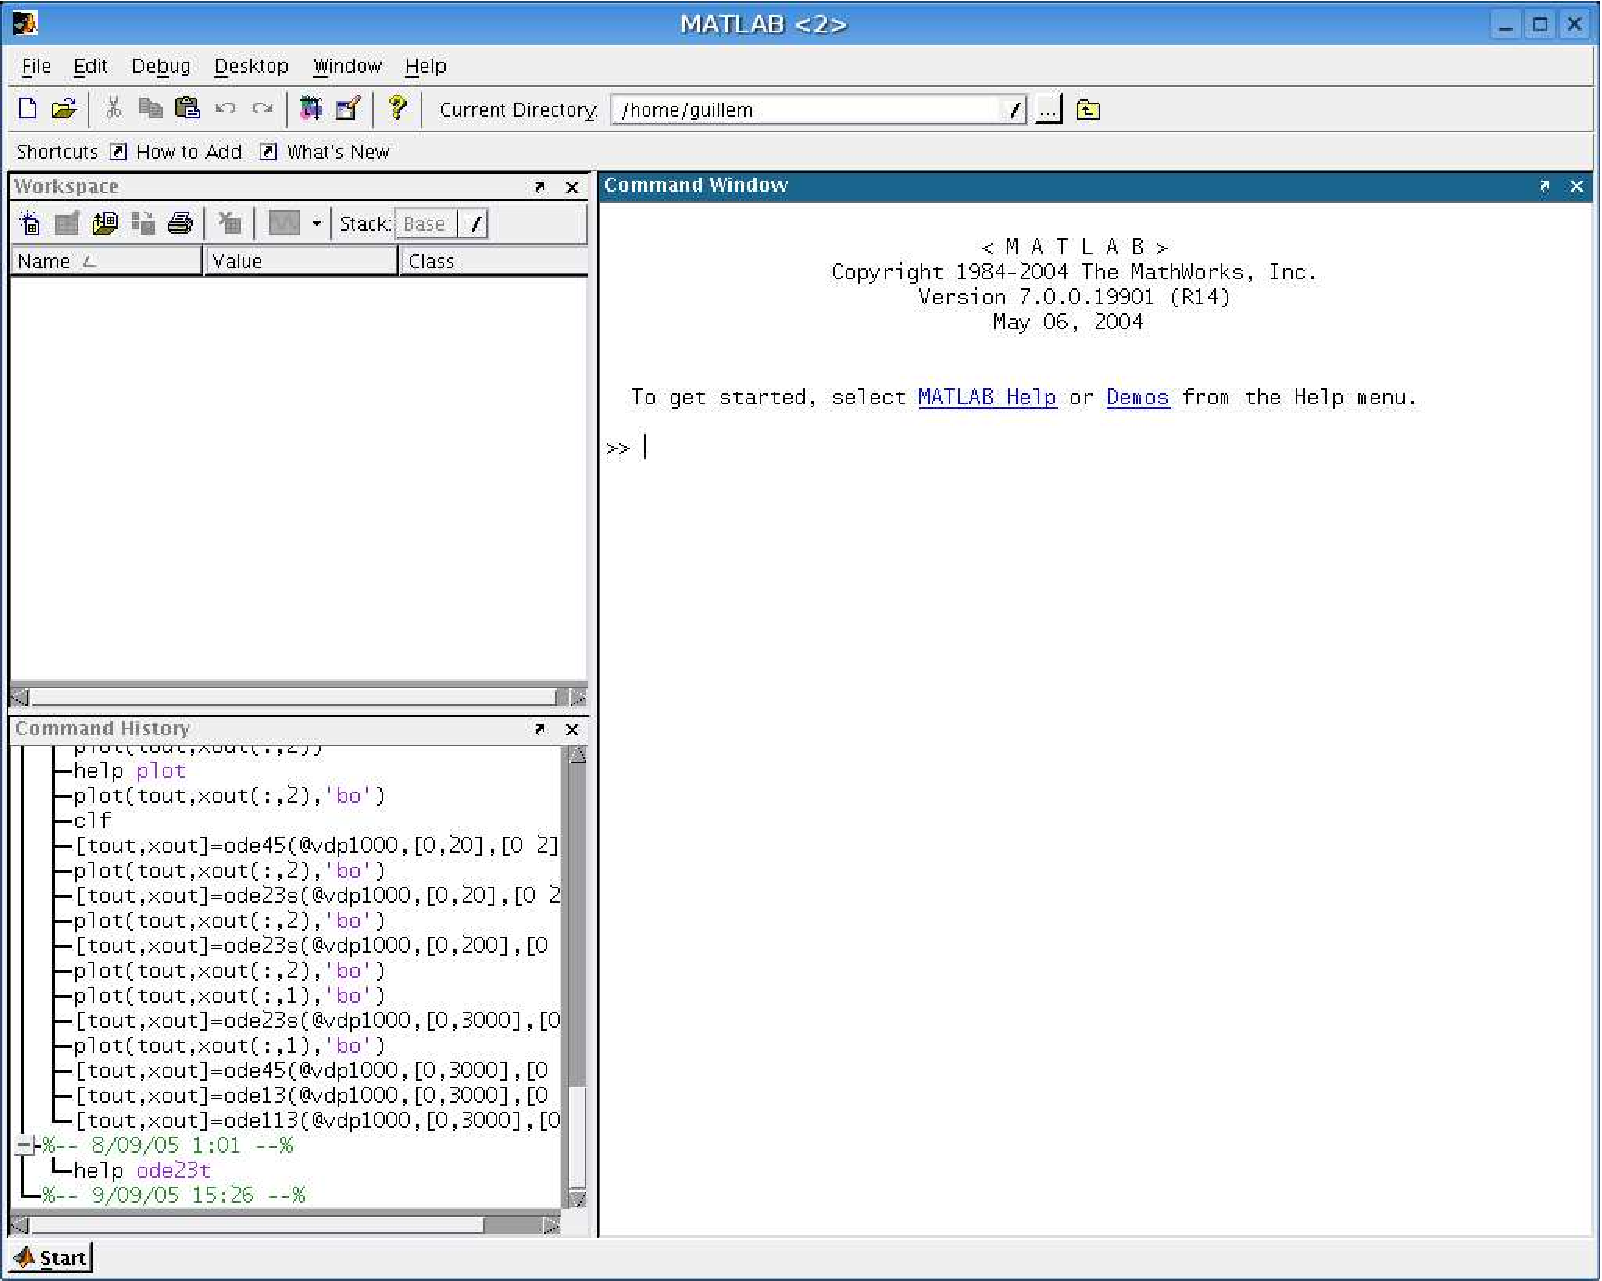
\includegraphics[ width=1\textwidth,
  keepaspectratio]{figuras/matlabenv}


  \caption{\label{cap:Ventana-principal-Matlab}Ventana principal de
    Matlab}
\end{figure}

La ventana principal no es más que la consola con algunas herramientas
adicionales. Para completar un entorno de desarrollo son necesarios
dos elementos más: un editor y un navegador de ayuda. El primero
aparece cuando editamos un archivo \texttt{.m} desde el gestor de
archivos o cuando creamos uno nuevo desde la ventana principal. Su
función es facilitar la creación de archivos de código Matlab y para
ello cuenta con {}``Syntax Highlighting'', tabulado automático,
soporte gráfico para debugging...

%
\begin{figure}[H]
  \centering{}

  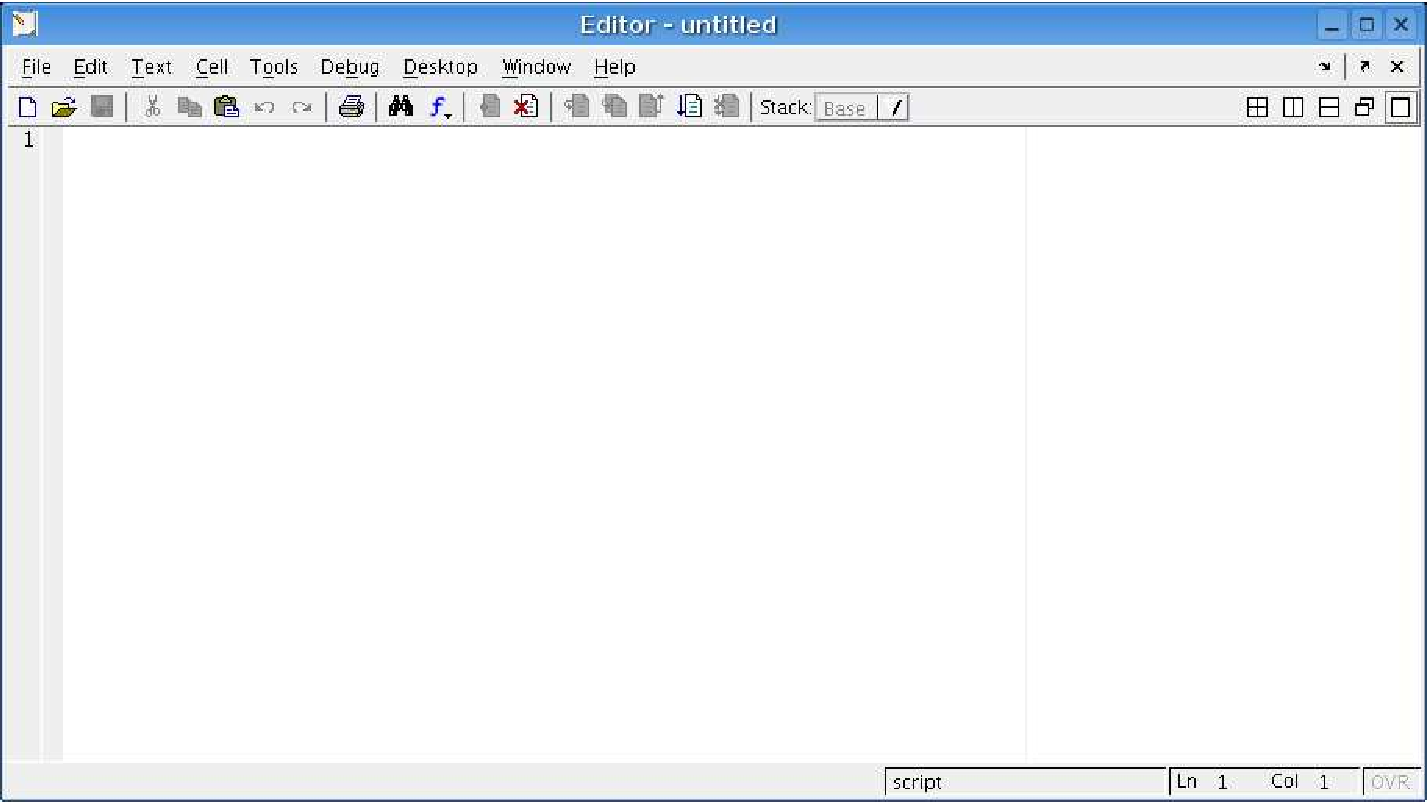
\includegraphics[%
  width=1\textwidth,
  keepaspectratio]{figuras/matlabed}


  \caption{\label{cap:Editor-Matlab}El editor de Matlab}
\end{figure}


Es muy importante llegar a dominar todas las posibilidades del editor.
Cuanto mejor lo conozcamos más fácilmente y rápidamente programaremos.

Finalmente el navegador de ayuda. Además de ser el mejor sitio donde
buscar ayuda puntual sus tutorías nos servirán para perfeccionar
nuestra habilidad con el lenguaje y el entorno. Podemos acceder a
él desde el menú {}``\texttt{Help}'' o mediante el icono con el
símbolo interrogante en la barra de herramientas.

%
\begin{figure}[h]
  \centering{}

  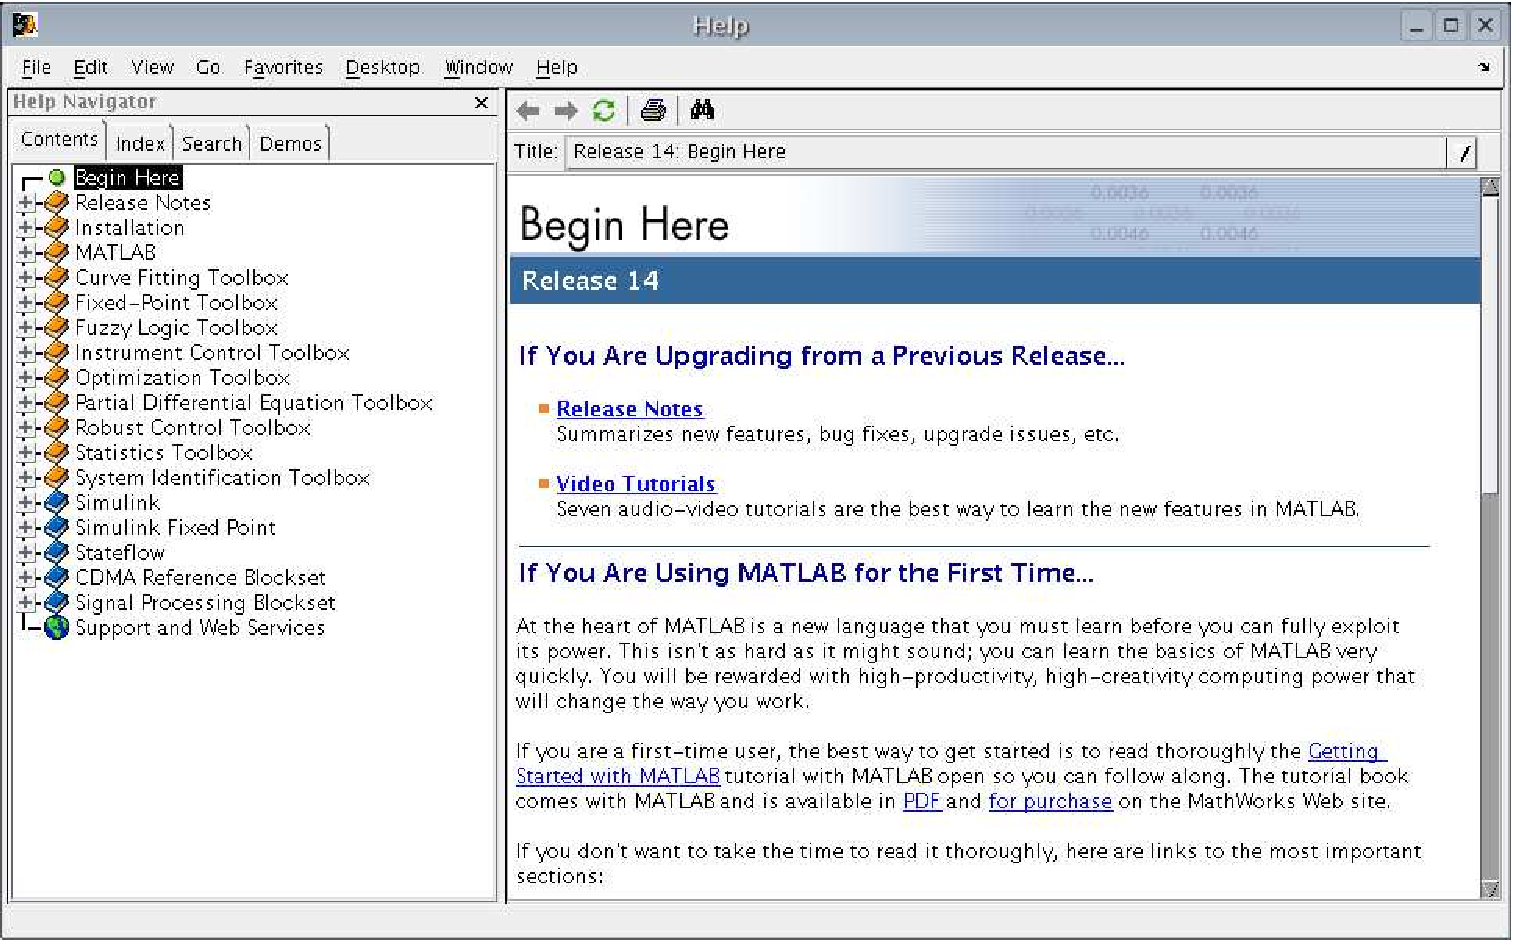
\includegraphics[%
  width=1\textwidth,
  keepaspectratio]{figuras/matlabhlp}


  \caption{\label{cap:Navegador-de-ayuda}Navegador de ayuda de Matlab}
\end{figure}



\section{Octave\index{Octave}}

Octave es también un lenuaje de scripting científico.  Aunque su
nacimiento nada tiene que ver con Matlab ha ido convergiendo hacia la
compatibilidad. Octave fue pensado como aplicación para la consola
UNIX. No tiene interfaz gráfica propia, navegador de ayuda, visor de
variables, editor, debugger...  Se puede decir que no tiene nada de
nada. Es un intérprete muy estable, ligero y orientado a programadores
más experimentados.

Octave es Software Libre soportado por una comunidad de
desarrolladores sin ánimo de lucro. Es un proyecto en colaboración
cuyos miembros nos prestarán ayuda cuando la solicitemos. Sus listas
de correo son públicas y son una gran fuente de información. Formar
parte del desarrollo de Octave es la mejor manera de conocer Matlab en
profundidad.

El lenguaje Octave es un poco más potente y mejor diseñado, si no nos
importa sacrificar la compatibilidad tendremos un poco más de libertad
programando.  Como parte del proyecto GNU su integración en un entorno
GNU/Linux es excelente; es por ello que se comunica perfectamente con
otros lenguajes de programación.  Puede ser una buena excusa para
perfeccionar o utilizar nuestros conocimientos de C++ o para
profundizar en UNIX.

Tampoco es verdad que Octave sea tan minimista. Existen esfuerzos para
dotar a Octave de más y más herramientas fuera del paquete oficial.
El más relevante es sin duda Octave-forge. Cualquiera que eche de
menos una función en Octave puede escribirla y mandarla al proyecto;
si lo creen conveniente la incorporarán en la próxima versión de la
colección. Además Octave-forge es un gran directorio de código
escrito. Puede servirnos para aprender como escribir una función como
es debido o como implementar algoritmos especialmente complejos. La
calidad de las funciones es variable pero la media es muy alta.

Otro proyecto interesante Octave Workshop de Sébastien Loisel.  Se
trata de una interfaz gráfica a la Matlab para Octave, orientada sobre
todo hacia usuarios de Windows.  Es un proyecto muy joven pero
prometedor; desde el principio ha apostado por una solución integrada.
Llena un vacío muy importante, de otro modo la curva de aprendizaje se
alarga por la necesidad de aprender a utilizar herramientas de UNIX en
un entorno Windows.

\subsection{El entorno de desarrollo Octave}

Cuando hemos hablado del entorno de desarrollo de Matlab han aparecido
tres ingredientes básicos: la consola, el editor y el naveador de
ayuda.  Como aplicación para la consola UNIX debemos confiar en las
herramientas propias del sistema: un editor polivalente como emacs o
vim, páginas de ayuda en formato info...  Aunque todas las piezas de
este entorno existen en Windows carecen de la misma integración con el
sistema operativo.  En este caso optaremos por un entorno de
desarrollo integrado como Octave Workshop.

El editor que mejor se complementa con Octave es Emacs (figura
\ref{cap:Emacs-editando-un}), parte esencial del proyecto GNU. Emacs
cuenta con un plugin para adecuarlo a la edición de archivos
\texttt{.m} y la comunicación con el intérprete Octave. Si no nos
sentimos cómodos con él siempre podemos optar por otros editores como
VIM o SciTe, este último muy adecuado para los usuarios de Windows.

El programa más utilizado para dar soporte gráfico a Octave es
GNUPlot.  Sus funcionalidades no son comparables a las ofrecidas por
Matlab pero son suficientes. Desde hace bastante tiempo se busca un
sustituto pero aún no ha aparecido ningún candidato adecuado.
Probablemente nuestra instalación de Octave incorpore GnuPlot, si no
es así tendremos que instalarlo puesto que es un requerimiento casi
indispensable.

Sobre el navegador de ayuda es muy conveniente obtener el directorio
de Octave-forge\index{Octave-forge}. Es un documento HTML comprimido
que cualquier navegador puede mostrar. No se acerca a las
posibilidades de la ayuda de Matlab pero es una buena herramienta de
consulta. En compensación, la ayuda interactiva de las funciones de
Octave suele ser de mayor calidad gracias al uso del formato
\emph{texinfo.}

%
\begin{figure}[h]
  \centering{}

  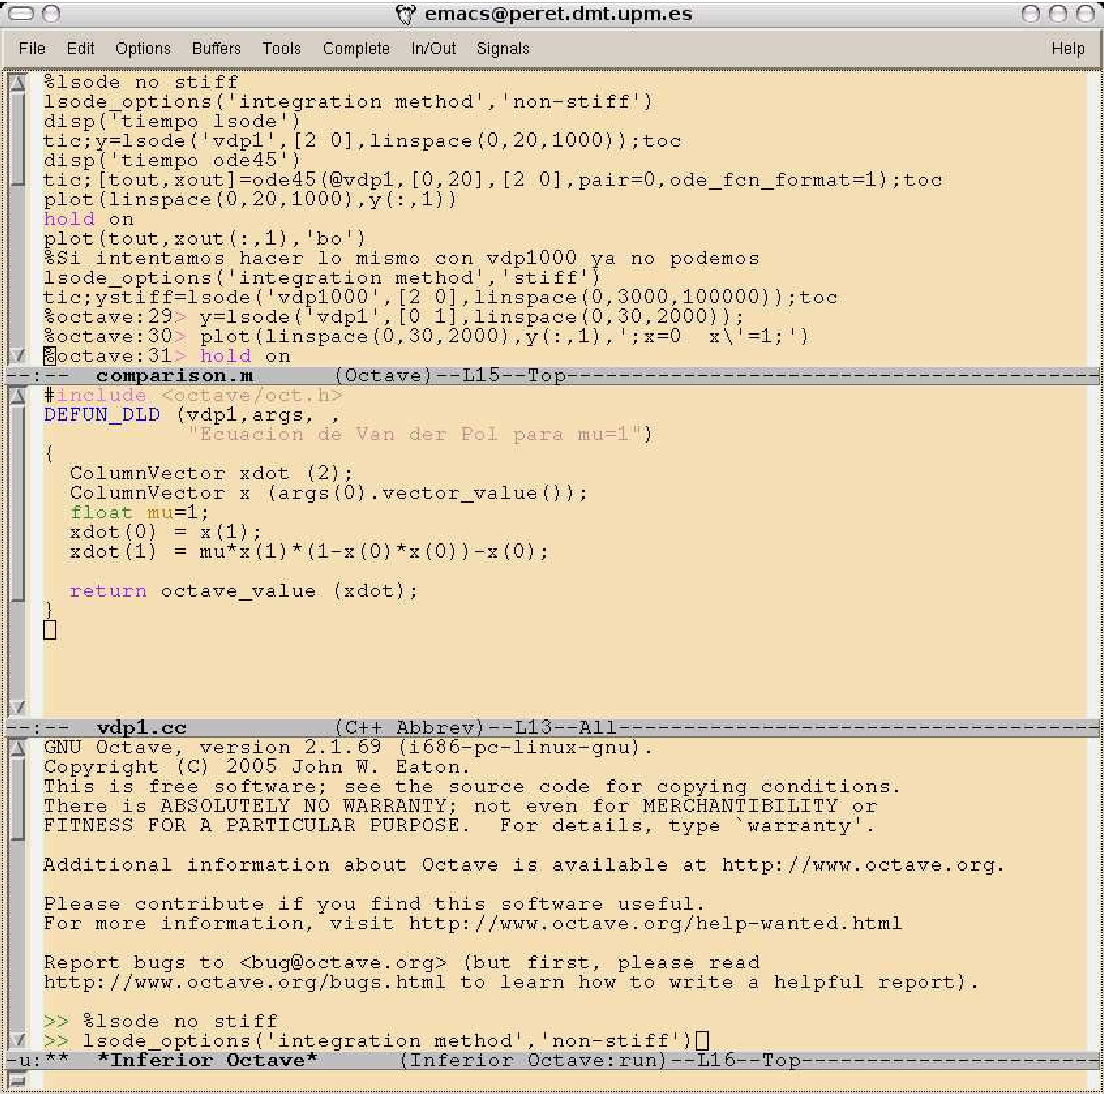
\includegraphics[%
  width=1\textwidth,
  keepaspectratio]{figuras/emacs}


  \caption{\label{cap:Emacs-editando-un}Emacs editando un archivo
    matlab, uno en C++ y debugeando simultáneamente.}
\end{figure}



\section{Los proyectos de software y los lenguajes de programación}

Cuando afrontamos un proyecto de software, sea del tipo que sea, la
primera consideración que se hace es la elección de la herramienta de
trabajo. En este caso un lenguaje de programación. Actualmente existen
un centenar de ellos y la elección no es sencilla.

¿Cuáles son los criterios principales?

\begin{itemize}
\item Que todos los miembros del proyecto dominen o conozcan el
  lenguaje.
\item El acceso a todas las herramientas necesarias.
\item El tiempo total de desarrollo del proyecto.
\item La calidad del resultado final.
\item La relación esfuerzo resultado.
\end{itemize}

Aunque estas condiciones parecen obvias no siempre han sido las
mismas.  Durante las décadas de los 70 y 80 programar se consideraba
una tarea laboriosa y complicada en la que no debía ahorrarse horas de
trabajo.  Que un ingeniero pasara miles de horas sentado delante de un
ordenador no se consideraba tiempo malgastado.  Existía la creencia de
que ninguna tecnología era capaz de competir con la pericia y que
cualquier aumento en el rendimiento compensaba con creces el tiempo
dedicado.

Durante los 90 aparecieron multitud de herramientas orientadas a
aumentar la productividad y con ellas un cambio esencial de filosofía.
El criterio era mucho más pragmático: todo cuenta.  Debemos valorar el
tiempo total de desarrollo, la calidad del código escrito, la
portabilidad del programa...  Ya no era sólo el programador y su
programa, se había convertido en una pieza dentro de una gran
maquinaria fuera consciente de ello o no.  La aparición de los
lenguajes interpretados acentuó aún más esta concepción.  Tareas que
antes llevaban días podían hacerse en horas y cada vez se hacía menos
necesario un conocimiento preciso de informática para programar.

El criterio esencial pasó de ser la calidad del resultado final a ser
la relación esfuerzo por resultado.  Los lenguajes interpretados suelen
mejorar dicha relación gracias a simplificar la metodología de
trabajo.

Hemos hablado de la distinción entre lenguajes de código fuente o
compilados y los lenguajes interpretados pero no hemos tratado sus
diferencias en el uso. Un lenguaje interpretado elimina la
necesidad del ciclo escritura-compilado-debugging.


\subsection{El ciclo de desarrollo clásico}

Todas las herramientas de desarrollo de software en general intentan
paliar los problemas derivados de este ciclo. Cuando programamos con
un lenguaje compilado como C o Fortran nos vemos obligados a convertir
el código fuente en un programa, ejecutar el programa, analizar el
resultado y, en el caso que sea necesario, realizar un debugging.  El
debugging es el proceso de depuración en tiempo de ejecución. Un
programa compilado se ejecuta entero y escupe un resultado final; si
no es el esperado y el código parece correcto nos veremos obligados a
analizar los resultados intermedios. ¿Cómo puede hacerse eso en un
ejecutable que parece un bloque monolítico? Introduciendo pausas en la
ejecución llamadas \emph{breakpoints} que paran el hilo para comprobar
los resultados intermedios.

Este ciclo es rentable sólo en el caso de grandes aplicaciones muy
integradas con las librerías o que requieren una máxima optimización.
¿Qué sucede si nuestra aplicación busca simple y llanamente un
resultado después de un tiempo de desarrollo lo más corto posible?
Entonces sacrificaremos los lenguajes de programación {}``clásicos''
en favor de los lenguajes interpretados


\subsection{Rapid Application Development o RAD}

La ventaja de los lenguajes interpretados respecto a los compilados es
evidente, uno de los pasos del ciclo de desarrollo, la compilación,
desaparece y el debugging es trivial. Esta diferencia que puede
parecer irrisoria suele condicionar enteramente el proceso.

Los lenguajes de scripting nacieron como una manera sencilla de hacer
tareas complejas o repetitivas. Por ejemplo, tenemos en un directorio
cualquiera medio centenar de archivos de los que no conocemos el nombre.
Nuestro objetivo es añadir al final de todos los que contengan la
combinación de letras \emph{abc} el símbolo \texttt{\_}. Realizar
manualmente esta tarea puede requerir unos cuantos minutos pero si
disponemos de un intérprete de \emph{python} en el sistema lo
conseguiremos con:

\begin{lstlisting}[language=Python]
>>> import os
>>> for file in os.listdir('.'):
...     if file.find('abc') >= 0:
...         os.system('mv %s %s%s' %(file,file,'_'))
\end{lstlisting}
Parece fácil. ¿Verdad? Si para los administradores de sistemas
conocer un lenguaje interpretado de propósito general es así de útil
¿Por qué no iba a serlo para un ingeniero? ¿Cuántas líneas de código
serían necesarias para programar lo mismo en C o Fortran?

Los ordenadores incrementan exponencialmente su potencia y cada año
los lenguajes interpretados son más y mas competitivos; ahora se usan
para casi cualquier aplicación y han obligado a todo el mundo a
cambiar su punto de vista. Los lenguajes interpretados se utilizaban
únicamente cuando se quería una interacción directa con el usuario,
una manera de extender las capacidades de un programa que estaba
escrito en un lenguaje compilado. Ahora podemos utilizar lenguajes
interpretados para aplicaciones de alto coste computacional y
pasaremos a un programa puramente compilado sólo en caso de necesidad.

Las aplicaciones de simulación suelen ser programas no muy largos que
pueden o no solicitar una optimización máxima. En cualquiera de los
dos casos se utilizará un lenguaje interpretado porque nuestro
objetivo es el RAD o Rapid Application Development. En programas
cortos porque es el único modo de acortar el tiempo de desarrollo y en
los largos para la fase de prototipado.

Para que un lenguaje interpretado pueda ser utilizado como una
herramienta de RAD debe cumplir los siguientes requisitos:

\begin{enumerate}
\item Debe ser lo suficientemente polivalente como para no necesitar acudir
  a otros lenguajes de programación durante del proceso de diseño.
\item Debe poner a nuestra disposición suficientes herramientas como
  para que no sea necesario \emph{buscar}.
\item Debe formar parte de un entorno de desarrollo cómodo, versátil
  y sencillo.
\item Su sintaxis debe ser clara para que el código sea leíble. En la
  mayoría de los casos los códigos se reciclan y mutan en el tiempo.
  Si cada vez que cambia de manos requiere ser leído cinco o seis
  veces para saber qué está haciendo es cualquier cosa menos rápido.
\end{enumerate}
Matlab cumple sobradamente todos estos requisitos. El lenguaje es
sencillo, cómodo y leíble; las bibliotecas de funciones son enormes y
siempre que no nos salgamos del cálculo numérico no tenemos que acudir
a otros lenguajes de programación.


\subsection{Otros lenguajes orientados a RAD.}

Matlab tiene competencia, esperada e inesperada. La esperada viene de
programas comerciales como Mathematica o Scilab. Además Mathematica hace uso de 
un concepto interesante conocido como Notebook, ya
introducido por Maple, para potenciar las sesiones interactivas. Lo
que probablemente no esperaban los desarrolladores de Matlab es que la
competencia les llegara por parte de los lenguajes interpretados de
propósito general.

Si nos obligamos a mantener el sentido crítico aplicado a las
herramientas debemos tener en cuenta lenguajes como Python o Ruby,
sobre todo Python gracias al proyecto SciPy. De momento son opciones
poco consolidadas pero puede que en un futuro sean una referencia en
el desarrollo de aplicaciones de simulación.

\section{Una visión contemporánea del desarrollo de aplicaciones de
simulación}

Es muy común que un ingeniero o un científico tenga que programar a
menudo. El desarrollo de aplicaciones de software está ligado a la
necesidad de simular un sistema de cualquier tipo. En la mayoría de
los casos los programadores son ingenieros, matemáticos o físicos sin
una formación teórica en lenguajes de programación. La mayoría de
ellos son autodidactas sin conocimientos específicos sobre metodología
y práctica de la programación. En muchos casos se construyen programas
deficientes con herramientas inadecuadas y del peor modo posible.  No
se usan bien los editores, los debuggers brillan por su ausencia, no
se aplican las metodologías orientadas a la programación sin errores...

La raíz de estos problemas es que el jefe del proyecto es el primero
en desconocer el entorno ideal. Casi siempre existen carencias en el
diseño de la aplicación y en la elección de las herramientas. ¿Cuántos
ingenieros han oído hablar del UML%
\footnote{UML son las siglas del Universal Modelling Language. Es un
  \emph{estándar} para la creación de diagramas que modelan la
  estructura de cualquier cosa, aunque fueron pensados para sistemas
  altamente lógicos como los programas de ordenador.%
}? ¿Y de la refactorización? ¿Cuántas aplicaciones de simulación están
escritas con un lenguaje orientado a objetos? ¿Y en un lenguaje
interpretado?  \emph{Los ingenieros somos tan soberbios como
  todoterrenos. Somos tan capaces de arreglar cualquier cosa como
  incapaces de reconocer que un mejor diseño nos ahorraría muchos
  quebraderos de cabeza}. En programas que requieren desarrollos de
horas o de días el coste de empezar de cero por culpa de un mal diseño
no es ningún problema; a medida que los tiempos de desarrollo crecen, la
situación se vuelve más y más crítica.


\subsection{Errores típicos}

El ingeniero tipo escribe un código lamentable, ilegible.
\textbf{Si en la construcción del ala de un
avión no se puede hacer una chapuza... ¿Por qué puede serlo el código
del programa que simula su inestabilidad?} ¿Por qué funciona? Otra
consideración fundamental es que si queremos producir una pieza
especialmente complicada construiremos antes un prototipo para saber
si cumple con los requisitos funcionales.  Si aplicáramos los mismos
principios al desarrollo de simulaciones sería intolerable ponerse a
escribir en Fortran más de 2000 líneas de código sin haber probado
antes el algoritmo en Matlab. Esta práctica es tan poco común en la
empresa como en el ámbito científico.

Otro error es el de subestimar el tiempo de desarrollo. Un programa de
simulación decente, con requerimientos computacionales medios o
grandes, puede desarrollarse en uno o dos años. Lo que suele hacerse
es tomar un lenguaje lo más rápido posible para minimizar el tiempo de
cálculo. Los lenguajes rápidos son principalmente dos, C y Fortran.
Normalmente se trabaja sin diseño, sin prototipos... Los errores
incomprensibles pueden alargar la aparición del primer ejecutable en
un 50\% del tiempo del proyecto, mucho más que lo que ahorraríamos en
el tiempo de ejecución.

Quizás la peor práctica de todas es la de no documentar el código a
medida que se escribe. Un código sin documentación o uno sin una
documentación adecuada puede ser un infierno hasta para uno mismo.  Si
leemos código escrito por nosotros mismos un año antes es como si lo
hubiera escrito alguien que no conocemos de nada. ¡Esto sucede de
verdad! Os lo digo por mi propia experiencia. Los comentarios son muy
útiles, hay que comentar cualquier estructura que no tenga una lógica
aplastante y escribir código obvio no es tan fácil como parece.


\subsection{¿Cuál es entonces el espacio de Matlab?}

Matlab es absolutamente superior en aplicaciones cortas y sencillas.
Reduce la longitud del código y el tiempo de desarrollo
significativamente además de ser un lenguaje leíble, escalable%
\footnote{Se dice que un lenguaje es escalable cuando todas sus
  virtudes se mantienen independientemente de la longitud del
  programa. Matlab es escalable pero hasta un límite; en aplicaciones
  especialmente grandes empiezan los problemas de uso de memoria y de
  acumulación de archivos de función. Los lenguajes compilados son
  típicamente escalables y algunos lenguajes interpretados como java y
  python también escalan perfectamente.%
} y sencillo. Todas las herramientas necesarias están dentro de la
misma aplicación y la documentación está embebida en el propio
programa%
\footnote{La ayuda de Matlab es un ejemplo de cómo se debe documentar
  una colección de funciones.%
}. Es una opción interesante en el proceso de diseño (cuando existe) y
es esencial en el proceso de análisis de datos, mucho menos exigente
computacionalmente.

La mayoría de los programas que escribe un ingeniero son cortos, y
requieren casi siempre las mismas herramientas matemáticas (álgebra
lineal, representación de funciones, integración numérica...). Se
busca efectividad, rapidez y pocos errores. Matlab es el lenguaje de
programación y la aplicación que mejor encaja en todos estos
requisitos en lo que a ingeniería se refiere.


\subsection{¿Y el espacio de Octave?}

Octave ha ido lentamente acortando las diferencias con Matlab. Hace
unos años no era más que una sencilla aplicación para la consola en
Linux.  Ahora, en su versión 3, es una aplicación multiplataforma con
una enorme biblioteca capaz de competir directamente con Matlab en
aspectos puramente técnicos.

Octave sigue siendo una alternativa a Matlab, pero una alternativa
cada día más seria.  Octave se usa activamente en los siguentes
entornos:

\begin{itemize}
\item En universidades de pequeño y medio tamaño, donde no se puede
  asumir el coste de las licencias de Matlab para todos los
  estudiantes de una aula de informática para las clases de cálculo
  numérico.  Es importante recordar que Octave nació en un entorno
  académico como herramienta de apoyo a los alumnos.
\item En empresas, también pequeñas y medianas, donde el coste de las
  licencias tampoco es asumible.  En este caso existe una tercera
  alternativa: la piratería. Octave tendría un impacto mucho mayor en
  este sector si pudiera darse a conocer de algún modo.
\item Octave sigue siendo una herramienta de uso personal para quien
  prefiere utilizar GNU/Linux.  En algunos casos por sencillez, en
  otros por una tendencia a utilizar herramientas libres.
\end{itemize}

Octave ha mejorado y sigue mejorando aunque este libro no sea capaz de
reflejar sus cambios.

\subsection{Los lenguajes \emph{pegamento}}

Otra característica de los lenguajes interpretados es que ellos mismos
están construidos sobre lenguajes compilados. Matlab, por ejemplo,
está escrito casi enteramente en C, mientras que Octave lo está en
C++. Esto significa que pueden integrarse perfectamente con sus
lenguajes \emph{padre}. Es de sobra sabido que los lenguajes
interpretados son entre uno y dos órdenes de magnitud más lentos que
los compilados.  La solución es acoplarles rutinas escritas en algunos
lenguajes compilados como C, C++ o Fortran para conseguir un aumento
significativo de velocidad.  Matlab empezó como una colección de
subrutinas en Fortran que se acoplaban a un intérprete interactivo.

Si este proceso se realiza sistemáticamente durante el desarrollo se
dice que el lenguaje interpretado sirve de \emph{pegamento} entre las
unidades de programa. Se puede decir que se buscan las ventajas de los
dos planteamientos, nos acercamos a la velocidad del código
enteramente compilado mientras mantenemos la versatilidad de un
script.

Matlab es capaz de convertir código en C o Fortran en archivos tipo
\texttt{mex} y Octave cuenta con el programa \texttt{mkoctfile}
(sección \ref{sec:Extender-Octave-con}) que realiza una labor
parecida. Lenguajes más polivalentes como Python, Ruby o
Perl cuentan con mejores herramientas.
